% !TeX spellcheck = pt_BR
% DO NOT USE \newcommand, \renewcommand, or \def.
% FOR FIGURES, DO NOT USE \psfrag or \subfigure.
% DO NOT USE \psfrag or \subfigure commands.

% jgrga JOURNAL OF GEOPHYSICAL RESEARCH
% gbc   GLOBAL BIOCHEMICAL CYCLES
% grl   GEOPHYSICAL RESEARCH LETTERS
% pal   PALEOCEANOGRAPHY
% ras   RADIO SCIENCE
% rog   REVIEWS OF GEOPHYSICS
% tec   TECTONICS
% wrr   WATER RESOURCES RESEARCH
% gc    GEOCHEMISTRY, GEOPHYSICS, GEOSYSTEMS
% sw    SPACE WEATHER
% ms    JAMES
% ef    EARTH'S FUTURE
% ea    EARTH AND SPACE SCIENCE

%%%%%%%%%%%%%%%%%%%%%%%%%%%%%%%%%%%%%%%%%%%%%%%%%%%%%%%%%%%%%%%%%%%%%%%%%
%  document
% \documentclass[draft,jgrga]{agutex}
\documentclass[jgrga]{agutex}
\usepackage[utf8]{inputenc}
% \usepackage[brazil]{babel}
%\usepackage[pdftex,plainpages=false,pdfpagelabels,pagebackref,colorlinks=true,citecolor=DarkGreen,linkcolor=NavyBlue,urlcolor=DarkRed,filecolor=Green,bookmarksopen=true]{hyperref}
%\usepackage[all]{hypcap}                    % soluciona o problema com o 
%\NeedsTeXFormat{LaTeX2e}
%\usepackage[T1]{fontenc}

%%%%%%%%%%%%%%%%%%%%%%%%%%%%%%%%%%%%%%%%%%%%%%%%%%%%%%%%%%%%%%%%%%%%%%%%%
% line numbers
% \usepackage{lineno}
% \linenumbers*[1]
%  To add line numbers to lines with equations:
%  \begin{linenomath*}
%  \begin{equation}
%  \end{equation}
%  \end{linenomath*}
%%%%%%%%%%%%%%%%%%%%%%%%%%%%%%%%%%%%%%%%%%%%%%%%%%%%%%%%%%%%%%%%%%%%%%%%%
% Figures and Tables
% [xdvi], [dvipdf], [dvipsone], [dviwindo], [emtex], [dviwin],
% [pctexps],  [pctexwin],  [pctexhp],  [pctex32], [truetex], [tcidvi],
% [oztex], [textures]
% \usepackage[dvips]{graphicx}
%\usepackage[dvipdf]{graphicx}
\usepackage{graphicx}
\usepackage{float}
\usepackage{multirow}
\usepackage{mathrsfs}
\usepackage{amsfonts}
%\usepackage{lipsum}

\usepackage{enumerate}
\usepackage{textcomp}
\usepackage{lmodern}

% print ilustrations on draft
\setkeys{Gin}{draft=false}


%-----------------------------------------------------------------------------
% glossaries
%-----------------------------------------------------------------------------
%
%\usepackage[acronym]{glossaries}
%\newglossary[slg]{symbols}{sym}{sbl}{Symbols List}
%\newglossary[elg]{equations}{eqn}{eql}{Equations}
%\makeglossaries

%---------------------------------------------------------------------------- 
% dicionary
%-----------------------------------------------------------------------------
%\input{d01-terms}
%\input{d02-symbols}
%\input{d03-acronyms}
%\input{d04-equations}
%---------------------------------------------------------------------------- 

%---------------------------------------------------------------------------- 
%  special operators
%-----------------------------------------------------------------------------
%\DeclareMathOperator*{\argmin}{arg\,min}
%\DeclareMathOperator*{\argmax}{arg\,max}
%\DeclareMathOperator*{\erf}{erf}



%% ------------------------------------------------------------------------ %%
%  ENTER PREAMBLE
%% ------------------------------------------------------------------------ %%


\lefthead{ASSUMP\c{C}\~AO \lowercase{et al}} 
\righthead{Terremotos: Eventos Raros}

% \afour

% dates
%\received{date received} 
%\revised{date revised} 
%\accepted{date accepted}

% publication
%\journalid{vol}{journal date} 
%\articleid{start page}{end page} \paperid{manuscript id}

% licence
% \cpright{AGU}{year} 
% \ccc{code}

\begin{document}
%% ------------------------------------------------------------------------ %%
%  TITLE
%% ------------------------------------------------------------------------ %%
\title{Terremotos no Brasil:\\
Preparando-se para Eventos Raros
}

%----------------------------------------------------------------------------------------
%	AUTHORS AND AFFILIATIONS
%----------------------------------------------------------------------------------------
\author{Marcelo Assump\c{c}\~ao	\altaffilmark{1}, 
		Marlon Pirchiner		\altaffilmark{1,2}, 
		Jo\~ao Carlos Dourado	\altaffilmark{3}, 
		Lucas Barros 			\altaffilmark{4} 
%    and Marcelo Assump\c{c}\~ao 		\altaffilmark{1}
		}
\altaffiltext{1}{Departmento de Geofísica, 
				Instituto de Astronomia, Geofísica e Ciências Atmosféricas (IAG),
				Universidade de S\~ao Paulo (USP), 
				S\~ao Paulo, SP.}
				
\altaffiltext{2}{Escola de Matem\'atica Aplicada (EMAp), 
				 Fundacão Getúlio Vargas (FGV),
				 Rio de Janeiro, RJ.}
				 
\altaffiltext{3}{Instituto de Geociências e Ciências Exatas (IGCE), 
				Universidade Estadual Paulista (Unesp), 
				Rio Claro, SP.}

\altaffiltext{4}{Observatório Sismológico (ObSis), 
				Universidade de Brasilia (UnB), 
				Brasilia, DF.}

%Corresponding author mailing address and e-mail address:
\authoraddr{Correspondentes: \\
			Marcelo Assump\c{c}\~ao (marcelo@iag.usp.br) e \\
			Marlon Pirchiner (marlon@iag.usp.br)
			}

%% ------------------------------------------------------------------------ %%
%
%  ABSTRACT
%
%% ------------------------------------------------------------------------ %%

% >> Do NOT include any \begin...\end commands within
% >> the body of the abstract.

\begin{abstract}

Há ocorrência de terremotos no Brasil. A ameaça e o risco são apresentados e possíveis correlações com a geologia são discutidas no contexto de sismicidade intraplaca. Uma proposta de quantificação da ameaça é apresentada e são discutidos algumas de suas etapas e conceitos. Definição e caracterização de fontes sismogênicas por zonas sísmicas e outros modelos de sismicidade suavizada assim como hipóteses usadas nos cálculos de ameaça são discutidos em maior detalhe. Resultados preliminares são apresentados e discutidos. Por fim, com suporte das últimas análises, são discutidos as formas mais adequadas para lidar com eventos raros e extremos como é o caso dos tremores de terra.

\end{abstract}

%% ------------------------------------------------------------------------ %%
%  BEGIN ARTICLE
%% ------------------------------------------------------------------------ %%


\begin{article}

%% ------------------------------------------------------------------------ %%
%  TEXT
%% ------------------------------------------------------------------------ %%
%------------------------------------------------------------------------------
\section{Terremotos no Brasil}
%------------------------------------------------------------------------------

%------------------------------------------------------------------------------
% \subsection{}
% \label{intro_intraplate_seismicity}
Sabe-se que o Brasil, por estar no meio de uma placa tectônica, longe das suas bordas, é uma região muito mais estável do que países andinos como Chile, Peru, Equador e Colômbia (Figura \ref{fig_sa}). Estes países estão na borda da Placa Sul-Americana onde o contato com outra placa em movimento (placa de Nazca) deforma a crosta e armazena altas tensões numa velocidade muito mais rápida do que no interior das placas. Geralmente essas tensões são liberadas repentinamente na forma de terremotos.  No Brasil, ocorre um sismo de magnitude $\geq$5 a cada cinco anos, em média. Na região andina, sismos de magnitude $\geq$5 ocorrem em média duas vezes por semana.  Isto dá uma idéia de quanto o Brasil é mais estável comparado às regiões mais ativas.

\begin{figure}
	\centerline{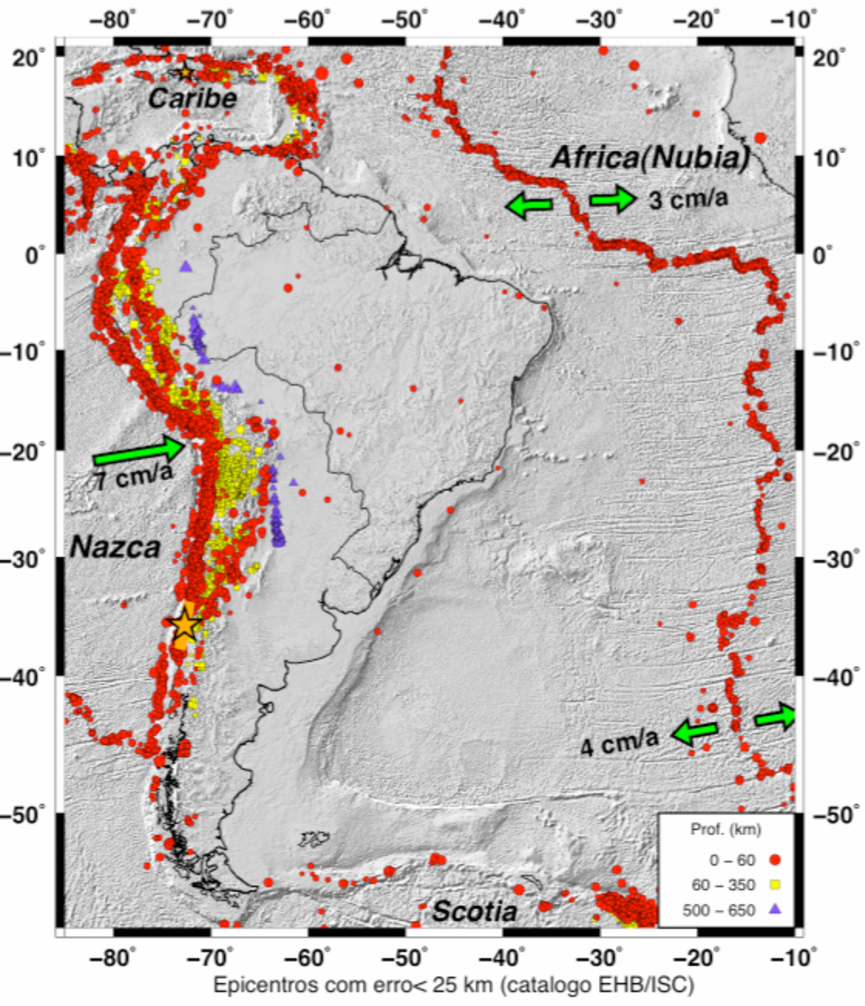
\includegraphics[width=\hsize]{img_america_do_sul}}
	\caption{Sismicidade na Placa Sul-Americana. Sismos do catálogo EHB do ISC (International Seismological Centre, UK) com magnitudes acima de 4.7 e incertezas epicentrais menores que 25 km. Setas verdes mostram o movimento relativo da Placa de Nazca e o afastamento da placa Africana na dorsal meso-oceânica.}
	\label{fig_sa}
\end{figure}


\begin{figure}[H]
	\centerline{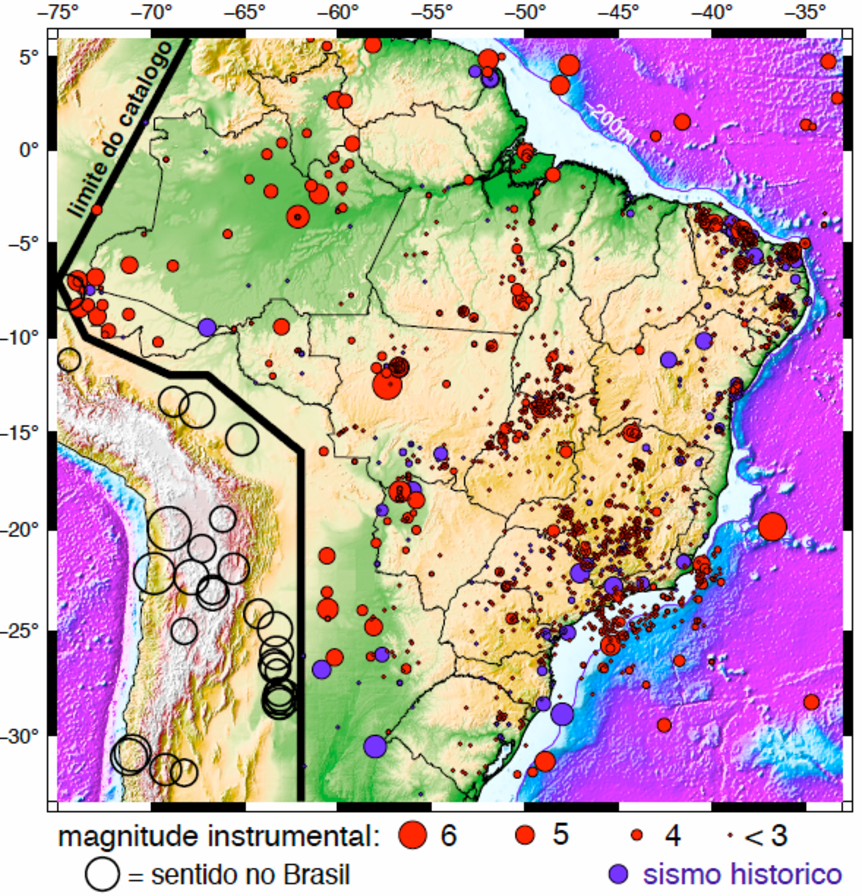
\includegraphics[width=\hsize]{img_bsb}}
	\caption{Boletim Sísmico Brasileiro \citep{bsb_2014} versão 2014.11. Círculos azuis são epicentros de sismos históricos com magnitudes estimadas pelos efeitos macrossísmicos. Círculos vermelhos são epicentros de sismos registrados por estações sismográficas. A região Sudeste, com maior densidade populacional e estações sismográficas há mais tempo tem sido melhor amostrada comparativamente a regiões mais remotas como a Amazônia.}
	\label{fig_bsb}
\end{figure}

Por outro lado, a Figura \ref{fig_bsb} mostra que sismos pequenos a moderados não são tão raros no Brasil. Sismos de magnitude 5 têm potencial para causar danos sérios em casas fracas, se o foco do sismo for raso e ocorrer próximo a regiões habitadas. Foi o que ocorreu em 09/12/2007 no município de Itacarambi, norte de Minas Gerais quando um tremor de magnitude 4,7 derrubou várias casas de construção precária matando uma criança. O mapa da Figura \ref{fig_bsb} mostra todos os tremores ocorridos no Brasil e já catalogados. Inclui sismos antigos estudados apenas através de relatos históricos assim como sismos recentes detectados por sismógrafos. Naturalmente já ocorreu um número bem maior de tremores no Brasil que não foram sentidos por terem sido em regiões desabitadas ou que não foram detectados por estações sismográficas por serem pequenos. No mapa da Figura \ref{fig_bsb} ainda é possível observar que a sismicidade não se distribui de modo uniforme espacialmente. A terra treme em algumas regiões com maior frequência do que em outras. 

O maior sismo do Brasil ocorreu no norte do Mato Grosso em 31/01/1955, a 1 hora da madrugada, com magnitude 6,2 (Figura \ref{fig_bsb}). Em Cuiabá, distante mais de 350 km do epicentro, várias pessoas acordaram com as vibrações sísmicas e saíram às ruas assustadas. A região epicentral (entre Porto dos Gaúchos e Sinop, MT) era desabitada na época. Uma repetição deste terremoto hoje certamente causaria sérios danos na área epicentral. Como comparação, o sismo de L’Aquila, Itália, em abril de 2009 teve magnitude 6,3 e causou muita destruição matando em torno de 300 pessoas. 

Em todo o Brasil, acredita-se que ocorram em média dois sismos por século de magnitude 6 ou maior. Nos Andes, magnitudes 6 ocorrem uma vez por mês. Por outro lado o excesso de confiança e a falsa sensação de imunidade pode ter um efeito surpresa aumentando as chances de negligência com os riscos envolvidos na ocorrência de eventos raros como tremores de terra. Ou seja, embora o Brasil tenha uma atividade sísmica muito baixa comparada a outros países de borda de placa, não está totalmente imune a tremores. A ameaça sísmica no Brasil é baixa mas não é nula e nem uniformemente distribuída!

\subsection{Risco e Resili\^encia: Frente a frente com Perigo}

O risco não é diretamente proporcional somente à magnitude dos eventos. Mesmo onde sismos são mais comuns como nas bordas de placas e onde sismos moderados já não são infrequentes, a raridade fica por conta dos eventos verdadeiramente catastróficos. Os riscos em um tremor catastrófico (magnitude acima de 8) são evidentemente diferentes no Chile e no Haiti por exemplo. É possível notar efeitos de ações de mitigação da vulnerabilidade e uma maior resiliência no primeiro. Sismos de magnitudes moderadas costumam causar mais perdas em locais menos preparados do que grandes tremores em locais onde já se espera que ocorram e trabalha-se para quando ocorram.

Há a necessidade de se preparar também para sismos intraplaca. Sismos moderados e fortes, embora ainda mais raros, quando ocorrem no interior de placas tectônicas podem ter muitos efeitos negativos devido principalmente à inadequação das estruturas. 

Dentre uma série de medidas possíveis para redução de danos e perdas, a sociedade pode valer-se de códigos e normas regulando os projetos de construções sismo resistentes onde e quando necessário. A severidade na exigência de parâmetros e projeto depende certamente da frequência de ocorrência destes fenômenos bem como do grau de risco aceito por cada sociedade. Como grande parte da ameaça e do perigo dos desastres naturais se dá por causas fora de alcance do controle humano, é preciso conhecer bem seus mecanismos para quantificar a ameaça dando suporte à ações de redução de vulnerabilidade e exposição. 

Compreender melhor a ameaça sísmica é tarefa fundamental. Apenas para se ter uma ideia quantitativa do significado de raridade no contexto sismológico brasileiro, suponha que os tremores aqui ocorram aleatoriamente em qualquer lugar. O histórico de sismos brasileiros indica que a ocorrência, devido a um sismo, de acelerações do chão capazes de provocar trincas em paredes numa localidade qualquer (nas capitais, por exemplo), superiores a 5\%g [porcento da aceleração da gravidade] é de apenas uma, em média, em cada mil anos. Mas o mapa da Fig. \ref{fig_bsb} mostra que os tremores não são espacialmente aleatórios. Há regiões bem mais ativas (como Ceará e Rio Grande do Norte, Sul de Minas, Pantanal, etc.) e outras bem mais calmas (como no meio das Bacias do Paraná e da Parnaíba). O problema é estar minimamente preparado onde e quando houver a próxima grande ocorrência.

\subsection{Sismicidade Intraplaca e Geologia}
No catálogo de sismos brasileiros (Fig. \ref{fig_bsb}) registrou-se um maior número de ocorrências em regiões mais habitadas e com mais estações sismográficas como o Sudeste. Em regiões como a Amazônia, historicamente menos habitada e monitorada, o número de sismos é menor mas contaminado pela ausência se registros e não necessariamente de eventos. Apenas com um catálogo mais ‘uniforme’ como o da Figura \ref{fig_bsb_uniforme}, onde apenas os sismos mais recentes e com igual chance de serem detectados em qualquer lugar do Brasil são representados, é possível eliminar o viés da detetabilidade na amostragem. A partir dele pode-se explorar quais são as áreas de maior e de menor atividade sísmica no Brasil com suas possíveis relações com as principais províncias geológicas.

\begin{figure}[H]
	\centerline{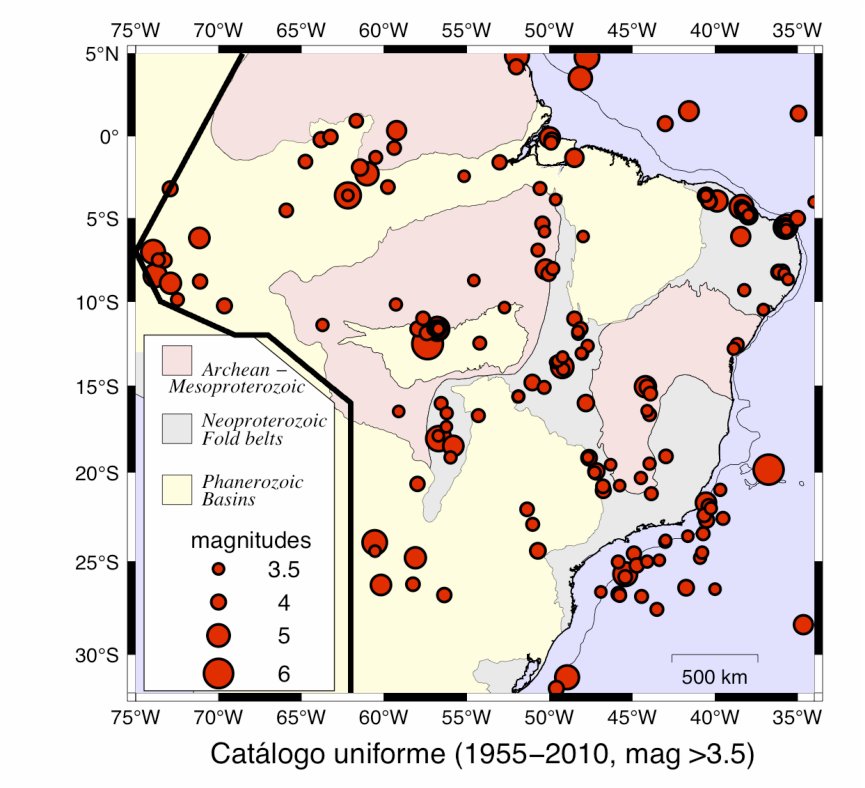
\includegraphics[width=1.17\hsize]{img_bsb_uniforme}}
	\caption{Catálogo uniforme, filtrado conforme detectabilidade: magnitudes $>$6 desde 1950; acima de 5 desde 1960, e acima de 3.5 desde 1980. O mapa mostra melhor as áreas de concentração de sismos e as áreas mais assísmicas.}
	\label{fig_bsb_uniforme}
\end{figure}

As relações entre sismos, estruturas e feições geológicas em regiões intraplaca são mais complexas do que se pode imaginar. Há pouco consenso entre especialistas sobre as causas da distribuição dos sismos.  A Figura \ref{fig_bsb_uniforme} mostra que não há uma relação muito óbvia entre áreas mais ativas e as províncias geológicas no Brasil: áreas cratônicas tendem a ser estatisticamente menos sísmicas, como mostrado por \citet{assumpcao_et_al_2014} e \citet{agurtodetzel_2015}. Entretanto há focos de sismicidade em interiores de crátons. O sismo de Itacarambi, MG, de 2007 ocorreu bem no meio do cráton do São Francisco, e o maior sismo conhecido no Brasil (Porto dos Gaúchos, MT, 1955) ocorreu no cráton Amazônico. 

Diferentes modelos geológicos têm sido propostos para explicar a concentração de sismos em certas regiões intraplaca baseados no conceito de zonas de fraqueza e concentração de tensões \citep{talwani_2014}. Mas embora grande parte os sismos intraplaca sejam rasos e ocorram principalmente na crosta superior (no Brasil a maioria dos sismos têm foco mais raso que 10 km) suas causas podem ser bem mais profundas. 

Entre os mecanismos tectônicos que podem concentrar tensões na parte superior da crosta estão:

\begin{enumerate}[a)]
	\item \textbf{afinamentos da litosfera} que tornam o manto litosférico mais fraco diminuindo sua capacidade de suportar as tensões regionais intraplaca. De acordo com \citet{assumpcao_2004} e \citet{azevedo_etal_2015} estas tensões acabam se concentrando na parte frágil da crosta superior. 

	\item \textbf{efeitos de flexura} devidos a carga de sedimentos ou a cargas internas da litosfera. Por exemplo, na faixa sísmica Goiás-Tocantins, região central do Brasil onde a crosta é mais fina, \citet{assumpcao_sacek_2013} sugeriram que o manto mais raso (e mais pesado) flexiona a placa para baixo causando tensões compressivas na parte superior da crosta. 
\end{enumerate}

Por outro lado, correlações diretas da sismicidade intraplaca com feições mapeáveis em superfície, como falhas geológicas e feições neotectônicas, têm se mostrado mais difíceis de interpretar. Por exemplo, o lineamento de Pernambuco, uma zona de cisalhamento várias vezes movimentada lateralmente desde o Brasiliano, é hoje uma feição sismicamente ativa sob esforços de tração Norte-Sul, sendo palco de pequenos falhamentos geológicos que podem ser de tipo normal ou transcorrente dependendo da orientação do ramo do lineamento em relação às tensões regionais conforme \citet{limaneto_etal_2013,limaneto_etal_2014}. No entanto a forte correlação entre o Lineamento de Pernambuco e a sismicidade no seu entorno é exceção. O Lineamento de Patos, por exemplo, não aparenta ter nenhuma relação direta com a atividade sísmica. Além disso a grande maioria dos tremores de terra no Brasil ocorrem sem nenhuma relação direta com feições mapeáveis em superfície segundo estudos de \citet{assumpcao_et_al_2014} e \citet{oliveira_etal_2015}.

\section{Proposta para um mapa brasileiro de ameaça sísmica}

Mapas probabilísticos de ameaça sísmica mostram os níveis de intensidade de movimentação do chão excedidos com uma certa probabilidade para um certo período de investigação.  Uma determinada intensidade de movimentação do chão (por exemplo, ``Peak Ground Acceleration'', PGA) em qualquer ponto do mapa pode acontecer devido a um tremor pequeno que ocorra próximo do local ou a um tremor maior porém mais distante. Um tremor grande e próximo também pode atenuar acima da média e ter pouca intensidade no local de interesse. Também é possível que um sismo pequeno, raso, em sedimento, amplifique acima da média provocando movimentos do chão com intensidades superiores às esperadas. Tudo isso deve ser levado em conta numa avaliação de ameaça.

As probabilidades de excedência de determinado valor de intensidade dos movimentos do chão dependem (1) da frequência anual de sismos de cada magnitude, e (2) de relações empíricas (``Ground Motion Prediction Equations'', GMPE) que estimam as acelerações em um certo local em função da magnitude de um tremor, da distância epicentral, das condições do solo no local, do regime tectônico da região do tremor, entre outros fatores. 

No cálculo da frequência de sismos (taxa anual de ocorrência), assume-se que no longo prazo os sismos continuarão ocorrendo com a mesma frequência registrada até agora em qualquer lugar dentro da zona sísmica. A maioria dos sismólogos acredita que áreas de maior atividade sísmica nas últimas décadas e séculos seriam locais mais prováveis para a rara ocorrência de um terremoto grande no futuro. Mas há quem discorde. Por exemplo, a área de Porto dos Gaúchos, no norte do Mato Grosso, que já teve sismos de magnitude 6 e onde continuam ocorrendo pequenos tremores ainda hoje (Figuras \ref{fig_bsb} e \ref{fig_bsb_uniforme}), em vez de ser uma zona de maior perigo, poderia ser um local onde as tensões já foram liberadas pelo terremoto de 1955. Por isso, talvez o próximo ‘grande’ terremoto brasileiro possa acontecer numa outra área aparentemente sem muita atividade sísmica recente, mas com muita tensão geológica acumulada e ainda não liberada. Esta situação de incerteza sismológica é pior onde as pesquisas geofísicas são muito recentes e os levantamentos geológicos incompletos, mas ocorre também em lugares onde levantamentos geológicos e geofísicos são bem mais detalhados. Uma discussão mais ampla sobre como lidar com essas incertezas foi apresentada por \citet{assumpcao_2011}. Apesar de controversa a abordagem mais tradicional e padrão na construção de mapas de ameaça sísmica é supor que os tremores continuarão ocorrendo nas mesmas zonas sísmicas como observado no passado. 

No Brasil já existe uma norma técnica da ABNT (NBR-15421/2006) \citet{nbr_15421_2006} que orienta o projeto e construção de edificações sismo resistentes. A versão atual da norma está baseada nos resultados do projeto mundial GSHAP (``Global Seismic Hazard Assessment Program'') apresentados por \citet{shedlock_tanner_1999} e reproduzido na Figura \ref{fig_gshap2}. 

\begin{figure}[H]
	\centerline{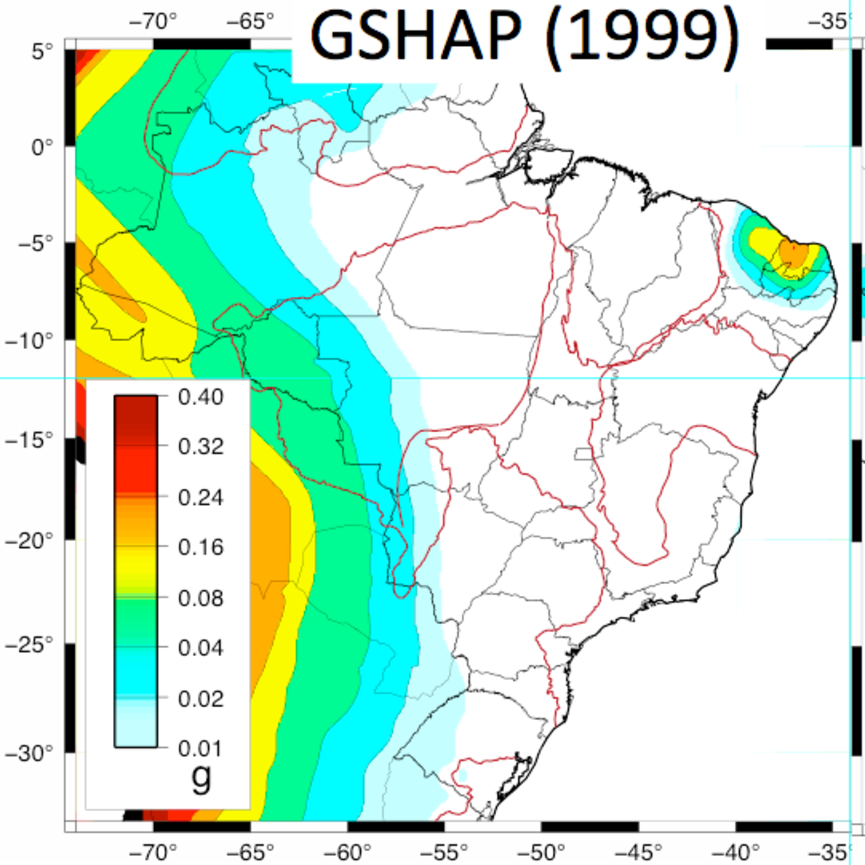
\includegraphics[width=\hsize]{img_gshap}}
	\caption{Mapa de Ameaça Sísmica (``Seismic Hazard'') do projeto GSHAP (Global Seismic Hazard Assesment Project, \citet{shedlock_tanner_1999}) usado como base para a norma sísmica brasileira, \citet{nbr_15421_2006}. As cores indicam as acelerações máximas horizontais (PGA, Peak Ground Acceleration) com probabilidades de 10\% de serem excedidas em 50 anos (i.e., com períodos de retorno de 475 anos). Linhas finas pretas são os estados, e vermelhas os limites das principais províncias geológicas do Brasil.}
	\label{fig_gshap2}
\end{figure}

A norma atual NBR-15421/2006 prevê na maior parte do Brasil acelerações menores do que 2.5\%g (para locais em rocha), com exceção de Ceará e Rio Grande do Norte, onde acelerações poderiam chegar a 5\%g.  Na parte oeste do Brasil, a influência da sismicidade andina poderia provocar acelerações até superiores a 10\%g, como no Acre. Estes valores referem-se à acelerações com probabilidade de excedência de 10\% em 50 anos (períodos de retorno de 475 anos).  Estudos mais detalhados da sismicidade do Brasil nos últimos anos sugerem que várias outras zonas sísmicas, como a região de Porto dos Gaúchos, norte de Mato Grosso, não foram consideradas como poderiam ter sido no projeto GSHAP e acabaram não sendo representadas no mapa da ABNT. Por esta razão um grande esforço vem sendo feito pela comunidade sismológica do Brasil (envolvendo USP, UnB, UNESP, UFRN, IPT, e PUC-RJ) para desenvolver um mapa brasileiro de ameaça sísmica. Serão apresentados alguns resultados preliminares.


\subsection{Delimitação de fontes sísmicas}

Como o conhecimento da sismicidade intraplaca ainda é incompleto e modelos diferentes são discutidos na literatura, a delimitação das fontes sismogênicas não é uma tarefa trivial e fácil. Para lidar com essas incertezas epistêmicas (falta de conhecimento da natureza) a melhor estratégia é levar em conta vários modelos possíveis, com seus pesos, numa árvore lógica. 


\begin{figure*}[t]
	\centerline{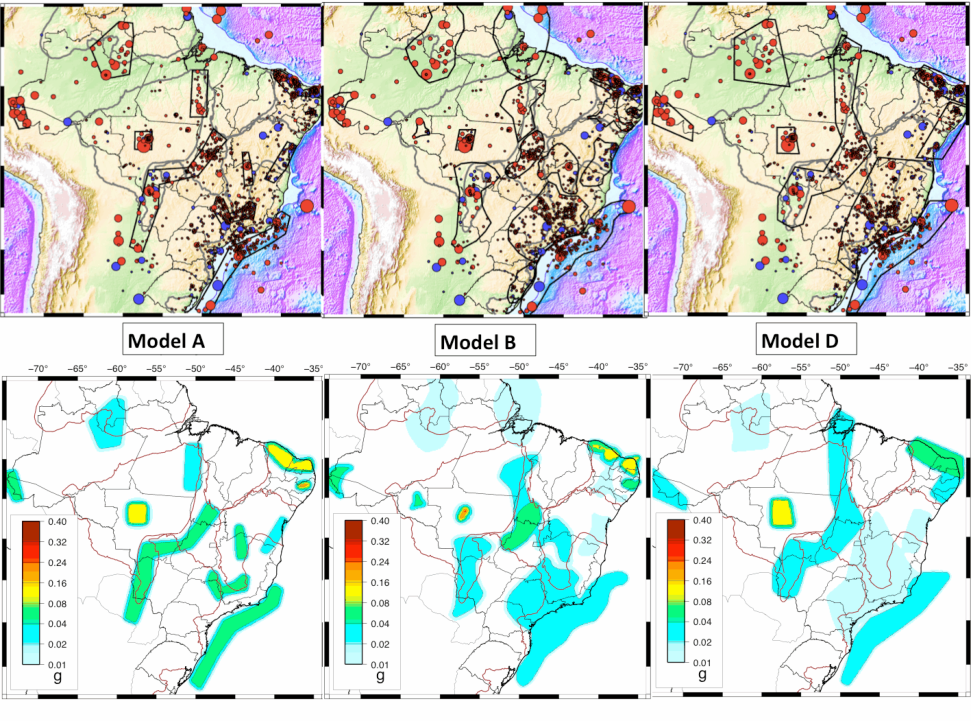
\includegraphics[width=\hsize]{img_zones}}
	\caption{Parte superior: três modelos de zonas sísmicas, segundo três especialistas diferentes. Parte inferior: mapa de ameaça resultante para cada modelo, com as acelerações (PGA) esperadas para 10\% de probabilidade em 50 anos.}
	\label{fig_zones}
\end{figure*}

A Figura \ref{fig_zones} mostra três modelos de zonas sísmicas, cada um proposto por um `especialista' segundo seus critérios e sua experiência. Nesta figura, apresenta-se também o mapa de perigo sísmico que resultaria de cada modelo de zoneamento sísmico. Nesta abordagem, a sismicidade é considerada uniforme dentro de cada zona sísmica. Isto é, calcula-se uma relação frequência-magnitude para os tremores dentro da zona (taxa anual de ocorrência = número de sismos por ano), e supõe-se que no futuro qualquer ponto dentro da zona tem a mesma probabilidade de ocorrência de sismos. Desta maneira, zonas sísmicas mais estreitas podem sobrestimar a ameaça sísmica, e zonas mais largas tendem a subestimá-la.

Uma outra abordagem possível é modelar a ocorrência dos sismos pontualmente, suavizando a própria distribuição dos sismos, em vez de zonas sísmicas em áreas pré-definidas. Mas precisam também de alguns parâmetros. Define-se uma grade cobrindo todo o país. O numero de eventos atribuído a cada ponto é o resultado somado da distribuição suavizada de cada evento em um entorno usando um kernel bidimensional \citep{frankel_1995}. Agora a taxa anual é definida como número de sismos por ano e por km$^2$. A Figura \ref{fig_woo} mostra um modelo onde a taxa de sismicidade em torno de cada ponto é calculada distribuindo os sismos ocorridos por um raio que depende do espaçamento médio entre os eventos de cada faixa de magnitude (método de \citet{woo_1996}). Existem inclusive modelos que suavizam a taxa de ocorrência em cada lugar usando um kernel de largura variável no tempo e no espaço \citep{helmstetter_2012}.

\begin{figure}[h]
	\centerline{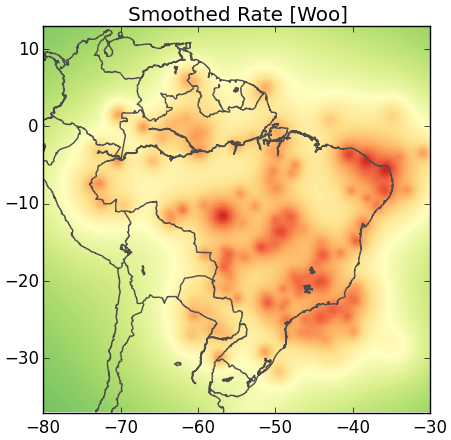
\includegraphics[width=\hsize]{img_rate_W}}
	\caption{Taxa anual de sismicidade (número de sismos por ano por km$^2$ com magnitude acima de 3) segundo o método de suavização de \citet{woo_1996}.}
	\label{fig_woo}
\end{figure}

\subsection{Modelos de Sismicidade}

Para construção de mapas de ameaça sísmica, inicialmente o catálogo de sismos do Brasil foi depurado eliminando clusters espaço-temporais de abalos precursores e réplicas. Isso é necessário já que os cálculos das probabilidades de ocorrência assumem que os tremores sejam igualmente aleatórios no tempo e no espaço. O que geralmente ocorre é que precursores e réplicas tendem a ocorrer no entorno de um tremor principal aumentando a taxa durante uma sequência sísmica e contaminando a média de ocorrências de magnitudes menores. Com essa depuração a distribuição da ocorrência dos eventos seguirá uma distribuição de Poisson. O mapa final de ameaça sísmica desconsidera os efeitos das possíveis réplicas e refere-se apenas ao sismo principal de cada sequência assumindo uma taxa de sismicidade constante que não varia no longo prazo.

Para cálculo das taxas de ocorrência (número de sismo/ano ou sismos/ano/km$^2$) foram estimados os períodos de completeza do catálogo sísmico. Isto é, para cada nível de magnitude, estimou-se a partir de quando o catálogo estaria completo. Isso varia em cada região do Brasil: no Sudeste e Nordeste, onde a população é maior, o catálogo está completo há mais tempo (por exemplo desde 1960 para magnitude acima de 3,5); já para a Amazônia o catálogo está completo há menos tempo (por exemplo, desde 1980 para magnitudes acima de 3,5). Na Figura \ref{fig_zones}, as taxas de ocorrência de sismos, para cada magnitude, foram calculadas para os três modelos de zonas de área. 

Adicionalmente foram usados três métodos diferentes de suavização: \citet{frankel_1995} com raio de busca uniforme de 110km, \citet{woo_1996} com raio variando com a magnitude (Fig. \ref{fig_woo}), e \citet{helmstetter_2012} onde o raio de busca variável depende da densidade de dados. 

Na árvore lógica foram atribuídos pesos iguais aos três modelos de zonas por área, e pesos de 21\%, 32\% e 47\% respectivamente, segundo testes, para os três métodos de suavização. O conjunto de modelos de fontes pontuais teve peso de 70\% e o conjunto dos três modelos de zonas por área teve peso final de 30\%.

\subsection{Modelo de Ameaça S\'ismica}

Fixada uma medida de intensidade, para um certo conjunto de valores possíveis, são calculadas as probabilidades de que o movimento do chão os exceda devido à ocorrência de tremores com magnitudes distribuídas de acordo com suas frequências e movimentando o chão segundo a distribuição de atenuações esperadas durante um certo período de tempo. Com isso é possível fixar uma determinada probabilidade (por exemplo 10\%) e mapear o valor de intensidade correspondente ou fixar uma intensidade (por exemplo PGA 0.1g) e mapear as probabilidades.  

As intensidades foram estimadas segundo a GMPE de \citet{silva_2002}.  Para o mapa de ameaça sísmica, tomou-se em cada ponto a média ponderada dos valores de aceleração como resultado da árvore lógica. Nestes mapas estão contempladas as contribuições à ameaça sísmica de sismos até magnitude 7, embora a contribuição principal seja de magnitudes na faixa de 5 a 6.


\begin{figure*}
\begin{tabular*}{\hsize}{
				p{0.5\hsize} 
				p{0.5\hsize}
				}
a) PGA, pde 10\% em 50 anos 
& 
b) PGA, pde 2\% em 50 anos 
\\ 
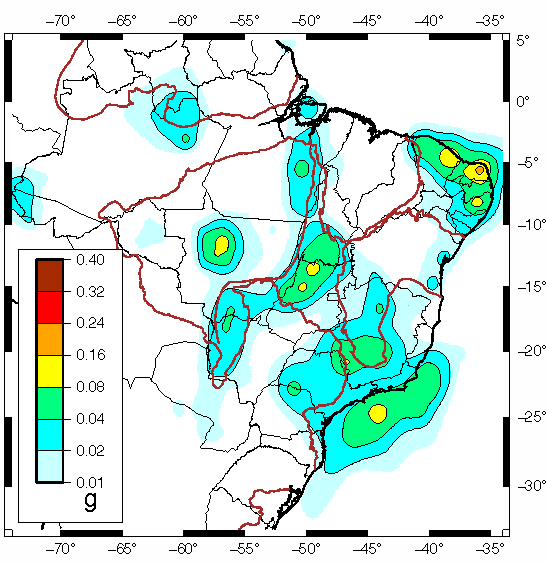
\includegraphics[height=\hsize]{img_hazard_10}
&
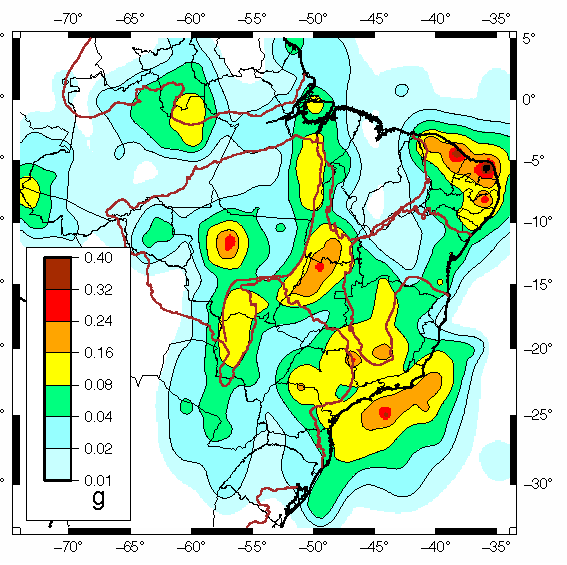
\includegraphics[height=\hsize]{img_hazard_02}
\\
\end{tabular*}
\caption{Mapas de Ameaça Sísmica (``Seismic Hazard Maps'') para aceleração de pico (PGA) em rocha, para probabilidades de 10\% (a) e 2\% (b) de excedência em 50 anos, correspondendo a períodos de retorno de 475 e 1475 anos, respectivamente. Cores são PGA em frações de g. Áreas verdes correspondem a PGA entre 4\% e 8\%g (equivalente a intensidades VI na escala Mercalli Modificada), áreas amarelas entre 8\% e 16\%g (intensidades VII MM).}
\label{fig_hazard}
\end{figure*}



Mapas preliminares de ameaça sísmica são apresentada na Figura \ref{fig_hazard}. Curvas de probabilidade (ameaça) foram calculadas para cada ponto do mapa. As Figuras \ref{fig_hazard}a e \ref{fig_hazard}b mostram as acelerações de pico (PGA) esperadas em local de rocha com probabilidade de excedência de 10\% e 2\% durante 50 anos (correspondentes a períodos de retorno de 475 e 1475 anos, respectivamente). Pode-se notar várias regiões do Brasil que apresentam acelerações esperadas acima de 3\%g (probabilidade de excedência de 10\% em 50 anos), preenchendo boa parte da área vazia do mapa GSHAP (Fig. \ref{fig_gshap2}) usado na norma vigente da ABNT. 


Este mapa preliminar ainda não leva em conta possíveis efeitos da sismicidade Andina, como se vê no mapa GSHAP (Fig. \ref{fig_gshap2}), o que deverá ser tratado na próxima versão. 

É importante ainda notar que, aparentemente, boa parte das construções críticas no Brasil, como as barragens de rejeito, estão projetadas para acelerações de 3 ou 5\%g. A extensão das áreas verdes das Figuras \ref{fig_hazard}a e \ref{fig_hazard}b sugere que estes valores poderiam ser revistos. 

\section{Eventos raros e extremos}

A principal diferença entre sismicidade de borda de placa (como nos Andes) e sismicidade intraplaca (como no Brasil), não é o nível das tensões geológicas existentes na litosfera (como se poderia pensar), mas a taxa de acúmulo de deformação e liberação em terremotos. Não há evidências de diferenças significativas nas magnitudes das tensões medidas na crosta. Pelo contrário, há indicações de que os sismos intraplaca liberam tensões um pouco maiores do que os sismos interplaca, na média. Isso implica em que terremotos grandes (magnitude 7, por exemplo) são apenas menos frequentes no interior das placas, mas não necessariamente impossíveis. Terremotos fortes intraplaca (magnitudes de 6 a 7) são eventos muito raros, mas possíveis.

Uma das grandes dificuldades de lidar com eventos geológicos muito raros (ou eventos extremos), é que o pouco que se conhece do passado geológico recente não é garantia de padrão para o futuro. Isso ocorreu com o mega-terremoto e tsunami da Sumatra em dezembro de 2004 que atingiu vários países matando cerca de 300.000 pessoas. Não se tinha conhecimento de nenhum outro tsunami parecido no oceano Índico. De um fenômeno que se repete a cada 300 ou 500 anos, em média, pode não se ter registros históricos suficientes. Mesmo no Japão, que conta com registros históricos muito antigos e um conhecimento geofísico bastante detalhado de todo o país, os sismólogos não achavam possível ocorrer uma ruptura tão extensa para que um terremoto atingisse magnitude 9, como o de Fukushima em 2011.  

O histórico de terremotos passados e os estudos da sismicidade atual não evitam surpresas num cenário de probabilidades baixas e baixíssimas. Sabe-se hoje que sismos de magnitude 5 a 6 podem ocorrer em qualquer região do planeta, mesmo no meio de uma placa tectônica e longe das suas bordas mais ativas. O tremor de magnitude 5,8 em 23/08/2011 na Virgínia, costa leste dos Estados Unidos, é outro exemplo recente. Não havia naquele estado nenhum registro histórico de tremores com magnitude acima de 5 (o último que havia provocado algum dano ocorreu em 1875 com magnitude 4,8).  

A melhor maneira de se minimizar as perdas devido a eventos muito raros, mas de consequências potencialmente catastróficas, tem sido avaliar adequadamente os fatores de risco e mitiga-los quando possível. E isso também depende de se quantificar a ameaça, ou as probabilidades condicionais de que esses eventos ocorram e, uma vez ocorrendo, de que tenham intensidade suficiente para afetar vulnerabilidades e provocar perdas e danos no ativo exposto. 

Mapas de ameaça sísmica são úteis para orientações em escala regional. Projetos específicos necessitam de avaliações específicas e individuais quanto mais elevados forem os riscos envolvidos. Para usinas nucleares, por exemplo, a prática internacional é adotar níveis de aceleração considerando períodos de retorno entre 10.000 e 100.000 anos. 

Certa resiliência pode ser alcançada por diferentes vias dependendo do quão aceitáveis são os riscos. O risco assumido, isto é, os valores das intensidades e probabilidades adotadas para cálculos estruturais em engenharia, depende dos requisitos de projeto. 

Equacionar o risco o custo e margem de segurança que se deve adotar é uma decisão da sociedade. Naturalmente, maior segurança implica em maiores custos que podem contribuir por exemplo com o aumento do preço de produtos e consequentemente dificultar a competitividade de setores como por exemplo o energético ou de mineração. 

A ciência e a tecnologia desenvolvem modelos quantitativos para avaliar a ocorrência dos eventos, seus efeitos e sua ameaça. À sociedade cabe discutir e regular os níveis aceitáveis de riscos inerentes aos empreendimentos e atividades de cada setor. Aos responsáveis por cada projeto, levando em conta a vulnerabilidade, a exposição e o risco, estimar possíveis perdas e seus custos de mitigação. O ponto de equilíbrio entre risco aceitável e custo é sempre uma decisão política conjunta.

\section{Conclusões}

A atividade sísmica no Brasil é baixa. Mas não sendo nula, a raridade do fenômeno aliada à falsa segurança devido à certa sensação de imunidade podem, por negligência, aumentar os riscos. Sismos médios e moderados (magnitudes até 5 ou 6) podem ocorrer em qualquer região mas com probabilidades tão pequenas que até agora foram consideradas suficientemente remotas tendo sido desprezadas na maioria dos projetos de edificações. O Boletim Sísmico Brasileiro \citep{bsb_2014} contém informação suficiente para um tratamento mais pormenorizado da ameaça sísmica brasileira do que estudos globais conhecidos. No Brasil, aparentemente, apenas instalações críticas, como usinas com reatores nucleares e barragens hidrelétricas, têm feito uso de análises sismológicas específicas. Quantificar adequadamente a ameaça sísmica é imprescindível para o correto dimensionamento dos riscos. Ainda, os estudos em andamento sobre a ameaça sísmica no Brasil e os resultados preliminares apresentados aqui sugerem que a norma sísmica atual poderia ser revisada contemplando acelerações de até 5\%g ou mais em áreas anteriormente consideradas `zona 0' e sem perigo apreciável.

%------------------------------------------------------------------------------
%	ACKNOWLEDGEMENTS
%------------------------------------------------------------------------------
\begin{acknowledgments}
Os autores agradecem a todos os colegas de trabalho e demais que de alguma forma colaboraram com o presente artigo.
\end{acknowledgments}

%------------------------------------------------------------------------------
%	BIBLIOGRAPHY
%------------------------------------------------------------------------------

\bibliographystyle{agufull08} 	% citação bibliográfica textual
\bibliography{bibliography}  	% associado ao arquivo:

%% ------------------------------------------------------------------------ %%
%	END ARTICLE
%% ------------------------------------------------------------------------ %%
\end{article}
\end{document}
